\documentclass[floatfix, aps]{revtex4-2}
\usepackage{natbib}
\usepackage[colorlinks=true, linkcolor=blue]{hyperref}
\usepackage{multirow}
\usepackage{float}
\usepackage{graphics}
\usepackage{tikz}
\usepackage{pgfplots}
\usepackage{amssymb}
\usepackage{amsmath}
\usepackage{graphicx}
\usepackage{gensymb}
\usepackage{siunitx}
\usepackage{rotating}
\usepackage{booktabs} % For better tables
\usepackage{listings}
\usepackage{color}
\usepackage{hyperref}
\usepackage{tabto}

\definecolor{listingkeyword}{rgb}{0,0,1}

\lstdefinelanguage{bash}{
  keywords={mkdir, cd, pwd, touch, echo, head, cp, mv},
  sensitive=true,
  morecomment=[l]{\#},
  morestring=[b]",
}

\lstset{
  language=bash,
  basicstyle=\ttfamily,
  showstringspaces=false,
  commentstyle=\color{red},
  keywordstyle=\color{blue},
  stringstyle=\color{teal}
}

\bibliographystyle{IEEEtranN}


\pgfplotsset{compat=1.18}

\begin{document}
\bibliography{Week1.bib}
\NumTabs{12}
\title{Intro2Astro - Week 1 Assignments}
\author{Kaushik P Palavalasa}
\date{\today}

\maketitle

\section{Assignment 1}

\subsection{Bash Script}
\begin{lstlisting}[language=bash]
#!/bin/bash
mkdir foo_dir 
pwd
cd foo_dir
touch week1.txt
echo "Hello, world" > week1.txt
head -n 10 week1.txt
cp week1.txt week1b.txt
mkdir foo_sub_dir
mv week1b.txt foo_sub_dir

\end{lstlisting}

\subsection{Unix Workbench and Data Carpentry}

\subsubsection{Unix Workbench}

\textcolor{blue}{\texttt{clear}} \tab - \tab 'clears' the terminal.

\textcolor{blue}{\texttt{echo}} \tab - \tab prints text to your terminal and other places as well using the \texttt{>} option.

\begin{figure}[H]
    \centering
    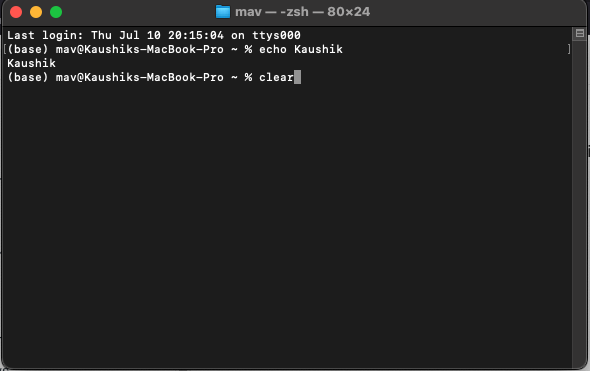
\includegraphics[width=0.75\linewidth]{Exercise 3.1 Unix Workbench.png}
    \caption{Solution to exercise 3.1}
    \label{fig:enter-label}
\end{figure}

\textcolor{blue}{\texttt{cd}} \tab - \tab changes the working directory which you can find using

\textcolor{blue}{\texttt{pwd}} \tab - \tab prints the working directory

\textcolor{blue}{\texttt{ls}} \tab - \tab lists all the files and folders in the working directory

\begin{figure}[H]
    \centering
    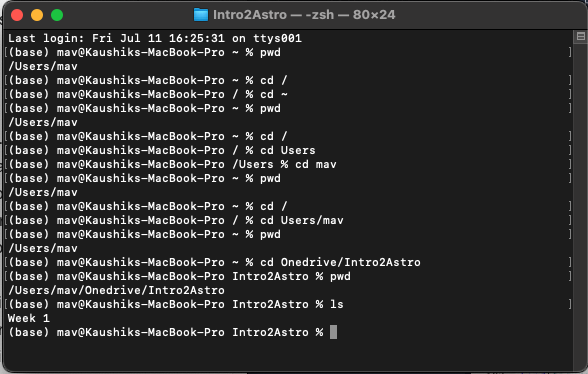
\includegraphics[width=0.75\linewidth]{Exercise 3.2.2 Unix Workbench.png}
    \caption{Solution to exercise 3.2}
    \label{fig:enter-label}
\end{figure}

\textcolor{blue}{\texttt{mkdir}} \tab - \tab makes a new directory inside the working directory

\textcolor{blue}{\texttt{touch}} \tab - \tab makes a new empty file

\textcolor{blue}{\texttt{>}} \tab - \tab redirects the output of a command into a file

\textcolor{blue}{\texttt{>>}} \tab - \tab appends the output of a command into a specified file

\textcolor{blue}{\texttt{cat}} \tab - \tab concatenates two files together, can also be used to display the contents of a single file 

\textcolor{blue}{\texttt{wc}} \tab - \tab print the number of lines, number of words and number of characters in a file, and the filename

\textcolor{blue}{\texttt{head}} \tab - \tab prints the first n lines of a specified text file

\textcolor{blue}{\texttt{tail}} \tab - \tab prints the last n lines of a specified text file

\textcolor{blue}{\texttt{less}} \tab - \tab allows you to navigate a long text file in the terminal

\begin{figure}[H]
    \centering
    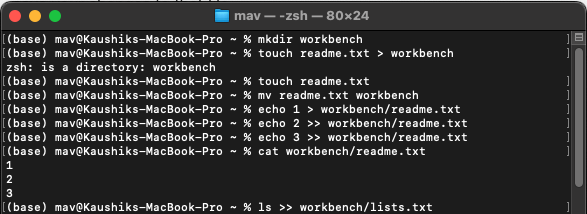
\includegraphics[width=0.75\linewidth]{Exercise 3.3.2 - 1.png}
\end{figure}

\begin{figure}[H]
    \centering
    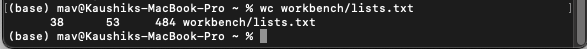
\includegraphics[width=0.75\linewidth]{Exercise 3.3.2 - 2.png}
    \caption{Solution to exercise 3.3 }
    \label{fig:enter-label}
\end{figure}

\textcolor{blue}{\texttt{mv}} \tab - \tab is used to move or rename files and folders

\textcolor{blue}{\texttt{cp}} \tab - \tab is used to copy files or folder

\begin{figure}[H]
	\centering
	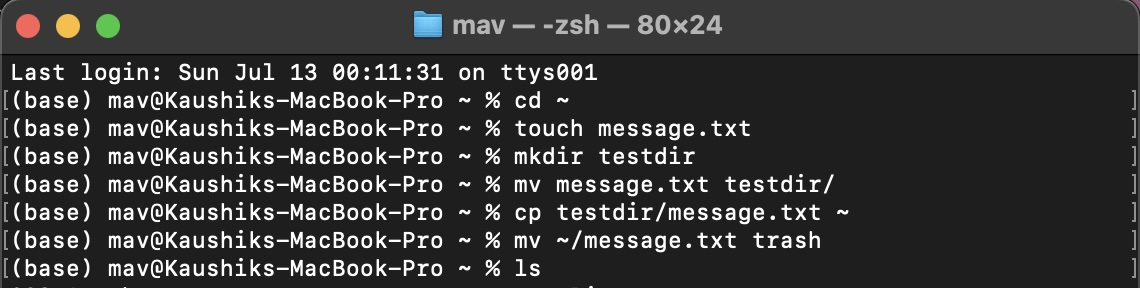
\includegraphics[width=0.75\linewidth]{Exercise 3.4 - 1.jpeg}
\end{figure}

\begin{figure}[H]
	\centering
	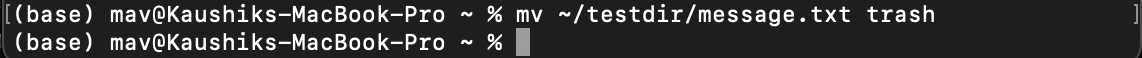
\includegraphics[width=0.75\linewidth]{Exercise 3.4 - 2.jpeg}
	\caption{Solution to exercise 3.4}
	\label{fig:enter-label}
\end{figure}

\textcolor{blue}{\texttt{man}} \tab - \tab prints the documentation for a command, that you can escape with \textcolor{blue}{q}

\textcolor{blue}{\texttt{apropos}} \tab - \tab prints a list of commands that are associated with the inputted word

\begin{figure}[H]
	\centering
	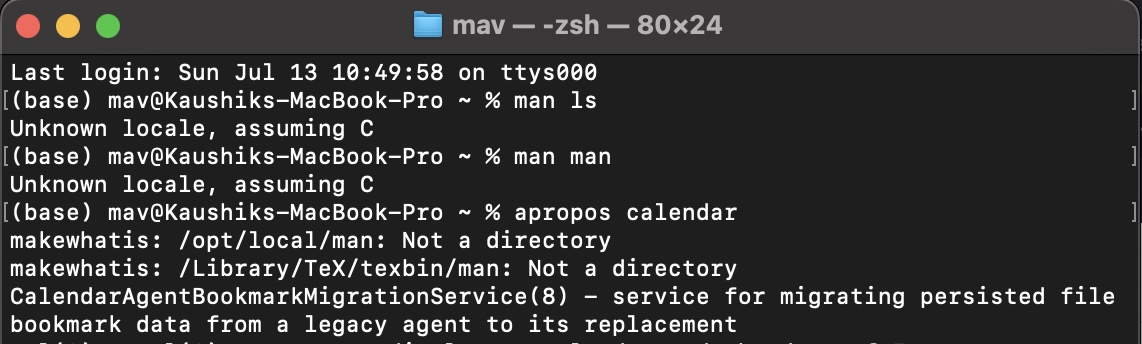
\includegraphics[width=0.75\linewidth]{Exercise 4.1 - 1}
\end{figure}

\begin{figure}[H]
	\centering
	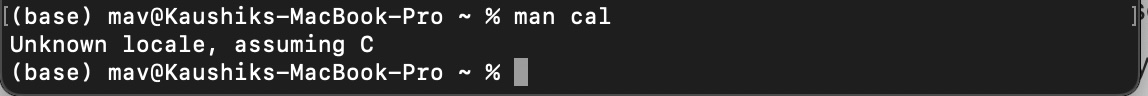
\includegraphics[width=0.75\linewidth]{Exercise 4.1 - 2}
	\caption{Solution to Exervise 4.1}
\end{figure}

\subsubsection{Data Carpentry}

\section{Assignment 2}

The paper that most directly proposes a novel method that could be utilized to attract the attention of, and communicate with extraterrestrial intelligence is \cite{Arnold_2005}. It suggests using Earth or Jupiter sized objects to create artificial dips in lightcurves which could then be used to transmit data. 


\bibliography{week1}


\end{document}